\chapter{Trade Study}
Portions of this chapter were originally compiled for the report, ``Enabling Technologies for Deep-Space Human Spaceflight: Human-Automation and Robotic Systems Trade Analysis'' by John Karasinski, Sherrie Holder, and Stephen Robinson, which was submitted to NASA in August, 2019.

% Enabling Technologies for Deep-Space Human Spaceflight
% Human-Automation and Robotic Systems Trade Analysis

% John Karasinski
% UC Davis PhD Candidate, NASA Ames Pathways Intern

% Sherrie Holder
% Space and Mission Critical Systems, The Charles Stark Draper Laboratory

% Stephen Robinson
% Professor and Director, UC Davis Center for Spaceflight Research

% August 21, 2019

% Abstract
% Appropriate integration between automation and robotics systems and their human operators is essential for future space exploration.
% The Human Factors and Behavioral Performance Element of NASA's Human Research Program requires a systematic understanding of the critical human-automation/robotic (HAR) integration, or HARI, design challenges for future space exploration.
% This document reports the results of a systematic assessment of the spaceflight-relevant HARI technologies and research topics addressing critical gaps in spaceflight-relevant HARI knowledge, and prioritizes the research required for successful human performance and HAR integration.
% We reviewed relevant literature across the past ten years and interviewed ten subject matter experts across industry and academia to investigate the current state of HARI technology, challenges facing development, the state of HARI research across a wide range of fields, and opportunities for advancing the state of the art through directed research.
% This information was used to identify relevant HARI technologies and research topics, as well as factors to assess relative priority of HARI technologies.
% We worked with NASA stakeholders to weight the factors relevant to assessing HARI specific technologies.
% A multi-dimensional trade analysis was performed to objectively score HARI research topics and specific technologies to recommended investment priorities for NASA.

\section{Executive Summary}
This investigation focused on a systematic assessment of current and upcoming human automation/robotic (HAR) integration, or HARI, technologies and research topics.
Analysis was focused on research and technology that address critical gaps in spaceflight-relevant HARI knowledge, and prioritizing the research required for successful human performance and HAR integration.
This is essential for NASA's Human Factors and Behavioral Performance Element to understand the critical human-automation/robotic integration design challenges for future space exploration.
A multi-dimensional trade analysis was performed to objectively score HARI research topics and specific technologies resulting in recommended research priorities for NASA investment.
A series of factors informing overall return on investment potential were used in weighted analysis of each technology.
Factors included characteristics such as TRL and applicability to relevant spaceflight tasks.
While these factors for assessment pertained directly to HARI technologies, research topics were assessed through direct relationships with those technologies (Figure~\ref{figure:tradestudyapproach}).

\begin{figure}[b!]
    \begin{center}
        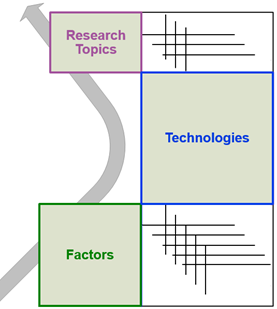
\includegraphics[width=0.49\textwidth]{figures/TradeStudy/figure1.png}
        \caption{Top-level trade study approach used in the HARI analysis}
        \label{figure:tradestudyapproach}
    \end{center}
\end{figure}
To understand the HARI trade space, we reviewed relevant literature across the past ten years and interviewed ten subject matter experts (SMEs) across industry and academia to investigate the current state of HARI technology, challenges facing development, upcoming automation/robotic technologies across a wide range of fields, and opportunities for advancing the state of the art through directed research.
Based on the gathered information, we derived a list of HARI research topics essential to addressing HARI development challenges and advancing the state of the art, as well as a list of specific HARI technologies with application toward HAR tasks common to either long duration deep space exploration (orbital) missions, space surface exploration missions, or both.
An initial set of factors for assessment of technologies was developed.
These factors were characteristics of technologies that effect the potential impact of development on NASA missions, or overall return on research investment.
Factors included HAR task applicability, task (capability) enabling, potential to reduce or introduce risk, and Technology Readiness Level (TRL), among others.

Factors were provided to a group of NASA HARI stakeholders from NASA Ames Research Center and NASA Johnson Spaceflight Center.
They were asked to review eight factors and rank them from most important to least important for consideration of HARI technology investment potential.
NASA stakeholders were informed that these factors would be weighted and used to conduct a trade study designed to help NASA prioritize which technologies and, consequently, which HARI research topics, should be pursued in support of future long duration exploration missions.
After gathering their input, the stakeholder's scores of the factors were averaged and ranked.
The final ranks were used in our trade analysis.

A multi-dimensional trade analysis was performed to objectively assess HARI research topics and specific technologies.
The factors for assessment were traded directly with HARI technologies, while research topics were assessed through direct relationships with those technologies.
Technologies were first assessed against each factor in a series of individual one-dimensional trade analyses (each trading technologies against one factor).
The results of these factor-level trades were normalized and used to score technologies, taking into account the relative factor weights, in the factor-to-technology dimension of the larger analysis (Figure 1).
The research-topic-to-technology dimension was assessed based on relationships between the two.
Research topics and technologies were defined as related if a given technology supports the research topic such that its development would fundamentally drive investigation of that topic.
The scores for each related technology for a given research topic were summed to achieve the total score for that topic.

The top-ranking research topics were: (1) Improving training for HAR systems and tasks, (2) Establishing appropriate trust in automation/robotics systems, and (3) Understanding human intent.
The top-ranking technologies identified from the trade study were: (1) Machine Learning, (2) Autonomous obstacle detection/imaging, (3) Robotic/human information interfaces, and (4) Artificial Intelligence.
These results reflect the surveyed background literature and the information gathered from our SMEs.
These top-ranking research topics were driven by their associated highly scoring technologies, while the top-ranking technologies have seen enormous advancements in research interest and development over the past few years, and all offer a large benefit to the tasks required by NASA on future missions.
The top-ranking technologies all benefited from high marks across all factors.

Based on the trade analysis performed, it is recommended that NASA prioritize research investment in the topics of improving training for HAR systems and tasks, establishing appropriate trust in autonomous/robotic systems, and understanding human intent.
These top-ranked research topics can be traced to trends of broad task applicability, high potential for risk reduction, low potential for risk reduction, and are areas whose study supports the advancement of research in lower-ranked topics as well.
Investigation of these research topics will provide a fundamental foundation for addressing challenges that face implementation of HARI technology solutions in future exploration missions.

\section{Introduction}
Technological advancements in automation and robotics necessitate appropriate integration between these systems and their human operators.
To date, there has not been a systematic evaluation of the HARI design challenges for human spaceflight critical to current and upcoming automation/robotic technologies.
Industries like transportation, air traffic management, and defense are investing significant time and effort to investigate and solve the many design challenges involved in human-automation/robotic integration.
NASA's Human Factors and Behavioral Performance Element needs to understand the critical human-automation/robotic integration design challenges for future space exploration.
A survey of the upcoming research topics and technologies which can be applied to NASA from a range of industries and domains is needed in order to reduce the risks associated with human spaceflight.

Therefore, an assessment of the upcoming technologies and open research challenges critical to effective human and automation/robotic integration (HARI) systems across industries and domains is essential to inform the design and development of safe, efficient future systems.
The objective of the current project is to conduct a systematic assessment of the space-relevant HARI automation/robotic technologies in order to prioritize necessary research required for successful human performance and HAR integration.
This includes identification of aspects that influence the relative importance of technology for spaceflight, or factors, for assessing prioritization of HARI related research and technologies.

\section{Project Background}
The overall objective of this study was to investigate HARI technologies on the horizon with the potential to support critical HAR tasks and use trade analysis to assess these technologies against critical factors for investment in order to determine recommendations for research and development.
The project was designed with two Phases, with Phase 1 focused on gathering background information and identification of specific technologies, and Phase 2 focused on trade analysis.
Tasks were originally proposed for each Phase as shown in Tables~\ref{table:phase1} and~\ref{table:phase2}.
This project largely followed the original two-phase plan, with background research informing the design of a trade study aimed to provide recommendations of technologies/research to pursue.
However, specific tasks were redirected, in coordination with the Human Automation / Robotics Integration (HARI) Discipline Scientist (DS) (NASA Civil Servant at Ames), as we gathered the background information in Phase 1 and learned more about the trade space.

In exploring HARI technologies and risks and challenges facing development, as described in the Phase 1 tasks, through literature review and interviews with Subject Matter Experts (SMEs), it became evident that technology implementations as described in Task 1.3 would vary widely due to dependence on specific mission design, even when constrained to a specific HAR task.
It would not be possible or practical to capture the space of all possible specific technology implementations at such a detailed level.
The primary goal of this project was to explore a trade space of HARI solutions or directions for research, not to trade on mission designs.
Rather than explore a subset of implementations whose applicability to a HAR task would be limited mission to mission, we chose to raise the level of the technology/research trade space and explore broader solutions to HARI challenges as they apply to HAR tasks common to the scope of long duration orbital and planetary surface exploration missions.
For example, exploring the potential of Augmented Reality/Virtual Reality (AR/VR) technology in general as applied to HAR tasks, as opposed to a specific implementation of AR/VR to train for surface operations that assumes a human-robot team makeup (a mission design decision).

In reviewing a draft of the report described in Task 1.5, it became apparent that the HARI solutions identified fell into two categories.
While some were technologies which support or enable HAR tasks, others were research topics related to those technologies whose study will fundamentally drive future HARI capabilities and directly address HARI challenges.
Given the importance of the research topics identified for addressing HARI risk, the trade analysis plan was directed to capture both technologies and research topics (and the relationship between them).
Additionally, with each technology and research topic applicable to a range of HAR tasks as described above, rather than having a separate analysis for each task, HAR task became a critical factor for comparison across the trade space, providing a more complete evaluation between technologies.
Although the process outlined in the Phase 2 tasks was followed, the focus of the trade analysis was shifted to reflect the nature of the trade space.
This shift allowed the study to produce relevant recommendations on closing HARI risk as intended.

\begin{table}[tb]
    \centering
    \includetable{hari-phase1.tex}
    \caption{Tasks initially proposed for Phases 1 of the HARI Trade Analysis}
    \label{table:phase1}
\end{table}

\begin{table}[tb]
    \centering
    \includetable{hari-phase2.tex}
    \caption{Tasks initially proposed for Phases 2 of the HARI Trade Analysis}
    \label{table:phase2}
\end{table}

\section{Background Research}
To begin the assessment of space-relevant HARI critical factors, we first completed a comprehensive literature review of the field of human and automation/robotics interaction.
Background literature primarily focused on survey papers from the past ten years, but also included prominent papers from noted authors in the field.
Primary research was also gathered from discussions with subject matter experts in human factors and human-robot interaction related fields.
Findings and lessons learned from this investigation are provided in this report.

\subsection{Literature Review}
We completed a review of human factors and automation/robotics integration survey papers published over the past decade, with an increased focus on the past five years.
Non-survey papers from highly cited and established experts were also added to this review to provide additional insights.
When reading these papers, care was taken to note recurrent topics and technologies that received specific focus, were forecast to generate additional interest in the near future or were otherwise noted as requiring greater study.

As a result of this literature review, major themes of in human and automation/robotic integration technology development and research were identified, see Table~\ref{table:key-papers}.

\begin{table}[tb]
    \centering
    \includetable{hari-key-papers.tex}
    \caption{Table of the key papers reviewed, and the topics discussed in each}
    \label{table:key-papers}
\end{table}

Each of these topics is briefly discussed below, referencing their fundamental papers when possible, as well as their forecasts from the previously reviewed articles.

\subsubsection{Machine Learning}
Machine learning (ML) is among the most commonly mentioned topics which authors forecast as being essential to the future of human-robotic interaction~\citep{wang_current_2018}.
Machine learning has enabled significant benefits in a variety of automation/robotics systems but has also given rise to the need for explainable systems and has raised additional questions about trust.
While machine learning techniques may be effective, they are rarely easily explainable, and operators often have difficulty understanding exactly why a system behaves as it does.
Additionally, as these systems have become more sophisticated, they have become able to continuously learn and update their behavior, making it challenging for operators to maintain both system understanding and appropriate levels of trust~\citep{chen_humanagent_2014}.

Machine learning techniques such as hidden Markov models, Gaussian mixture models, and radial basis function neural networks, though usually requiring a supervised training phase, have been shown to be very effective in predicting human intent in the context of physical human-robotic interaction~\citep{losey_review_2018}.
In reviewing which machine learning algorithms are currently being used, Zamora et al. found that neural networks accounted for an overwhelming majority, but that both supervised and unsupervised algorithms were about equally common~\citep{zamora_machine_2017}.
ML is essential to the fields of vision-based hand gesture recognition and non-visual gesture recognition, without which gesture recognition devices would be impossible~\citep{liu_gesture_2018, rautaray_vision_2015, 8701742}.
As computer technology continues to rapidly advance, the ability to detect, track, and classify gestures in real-time has enabled this technology to be implemented in manufacturing and other industrial plants.
Liu et al. specifically call out a need to combine different ML algorithms to improve efficiency, and that deep learning techniques are now enabling non-wearable sensors~\citep{liu_gesture_2018}.
ML has also been used to vary the personality and behavior of adaptive social robots~\citep{ahmad_systematic_2017}.

In her 2017 paper, Endsley noted the research needs for the next thirty years of designing and building fully autonomous systems~\citep{endsley_here_2017}.
Several of these specifically concern machine learning techniques, including validating autonomy software, learning system consistency and transparency.
There are currently no effective techniques for validating autonomy software, as ``traditional methods fail to address the complexities of learning systems.
Exhaustive testing of rules and potential system states will not be possible and understanding boundary conditions will be difficult"~\citep{endsley_here_2017}.
Validating machine learning solutions is currently an active area of research.
There is concern about consistency in learning systems, as different systems will learn using different techniques and provide different levels of feedback about how their automation has changed based off new data.
Endsley notes the lack of transparency in learning systems as a unique challenge, saying ``[t]he actual logic and lessons 'learned' by neural networks and deep learning software are typically opaque not only to the human operator but also to software developers who may not fully understand how the system will behave in all circumstances"~\citep{endsley_here_2017}.
These problems are exemplified by Sheridan, who notes that ``[i]t is becoming clear that many complex traffic situations are exceedingly difficult for computer vision and artificial intelligence to 'understand' and that many accidents are avoided by social interaction between drivers, such as mutual eye contact, hand signals, and so on.
Understanding the social aspects of driving in traffic, as well as the degree to which cars can be safely automated, demands much further research"~\citep{sheridan_humanrobot_2016}.

\subsubsection{Flexible, Adaptive, or Adaptable Automation}
Flexible, adaptive, and adaptable automation are widely praised in the literature for their ability to provide dynamic levels of automation.
The flexibility to provide different sets of automated features during different mission phases, for instance, is an effective requirement for many modern tasks.
One example of this is the autopilot software used in modern transport aircraft, which includes multiple modes of automation for takeoff, cruise, and landing.
Chen and Barnes define flexible automation as ``systems that invoke various levels of automation depending on the operator's state, critical events in the environment, or algorithms related to specialized problem sets"~\citep{chen_humanagent_2014}.
Chen and Barnes and others have subdivided flexible automation into subtypes, based on the involvement of humans in the decision making process: adaptive automation—where tasks are assigned using conditions established before a mission, adjustable automation—where the human decides when to invoke automation, and mixed-initiative systems—where both the human and the system jointly decide how to allocate tasks~\citep{chen_humanagent_2014, beer_toward_2014}.
These dynamic changes in the role of the human in the human-automation interaction are meant to ``either increase the robot's level of autonomy at the expense of the human's authority, or, conversely, increase the human's control over the shared cooperative activity at the expense of the robot's autonomy"~\citep{losey_review_2018}.
These systems help maintain overall performance while attempting to reduce workload and maintain situational awareness for their human operators~\citep{kaber_situation_2006}.

Among these three automation technology areas, adaptive automation has seen the most research, and many authors have involved it in empirical studies~\citep{vagia_literature_2016}.
The primary difficulty with adaptive automation lies in ``thorny human factors issue of [function] allocation...which has been met with marginal success"~\citep{vagia_literature_2016}.
Optimal assignment of tasks between the operator and the system is difficult as it requires excellent understanding of the performance of the operator and the system's response to the operator.
It also requires the operator to be fully aware of the functional allocation at all times, otherwise mode confusion may occur.

Flexible automation can react to dynamic changes in the environment, and researchers have been able to include real-time sensor data of human physiological states to bring the operator's workload and situational awareness into the loop.
Monitoring the human allows the system to automatically take over tasks when workload is high, and has been used to send control back to the human when the system notes that they have become complacent or as an attempt to increase situational awareness~\citep{lu_human_2016}.
This type of automation is already present in self-driving vehicles on the road today—self-driving vehicles require that drivers have their hands on the wheel even when in self-driving/lane-keeping modes.
While this flexible automation is often effective in common and well understood systems such as driving, there is some concern that flexible automation may prove detrimental in complex and potentially unpredictable systems such as robotic swarms~\citep{kolling_human_2016}.

While adaptive and adaptable automation has been the subject of many experiments over the past few decades, the question of who should be in charge of setting the level of automation remains an open question in need of further study, though mixed-initiative systems may provide the best of both worlds~\citep{chen_humanagent_2014, parasuraman_humans:_2008}.
Chen and Barnes conclude their review by noting that ``[m]ixed-initiative architectures take advantage of the synergy between the more sophisticated worldview of an experienced human as well as the agent's logical precision and more rapid latencies"~\citep{chen_humanagent_2014}.
This architecture is inherently complex and difficult to study, however, as individual differences such as age, expertise, and trust have large effects when interacting with these systems~\citep{schaefer_meta-analysis_2016}.
Further research is recommended into different types of flexible automation, especially when it deals with very complex systems.

\subsubsection{Networked Multi-robot Systems and Swarms}
Human automation/robotics interaction has traditionally focused on a single robotic system, but the miniaturization of computer technology has made swarm or multi-robot systems an increasingly viable option.
The ability for swarms to dynamically reconfigure themselves in response to changing environmental variables and task demands, however, can lead to complex requirements on the human operator.
There remain important questions to be answered in the realm of human systems integration with swarms, especially regarding human supervisory control~\citep{kolling_human_2016}.
There is a specific concern with monitoring human workload and situational awareness as the number of robots increases.
Depending on the number and ability of robots and the type of tasks being performed, it is possible to quickly overburden the swarm operator, especially when operator is required to negotiate swarm-swarm interactions.
Kolling et al.'s 2016 review breaks the cognitive complexity of the human-robot system into three complexities: robots performing independent activities, with complexity O(n), which allows more robots to be controlled simply by adding more operators in a linear manner; robots interacting with other robots fully autonomously, with complexity O(1), which allows for a fixed number of robots to control any number of robots; and the case where robot-robot interaction must be controlled by an operator, with complexity O(>n), as the dependencies between robots results in more demand faster than the number of robots grows~\citep{kolling_human_2016}.
See Figure~\ref{figure-hari:controlcomplexity} for a graphical illustration of control complexity under each of these conditions.

\begin{figure}[b!]
    \begin{center}
        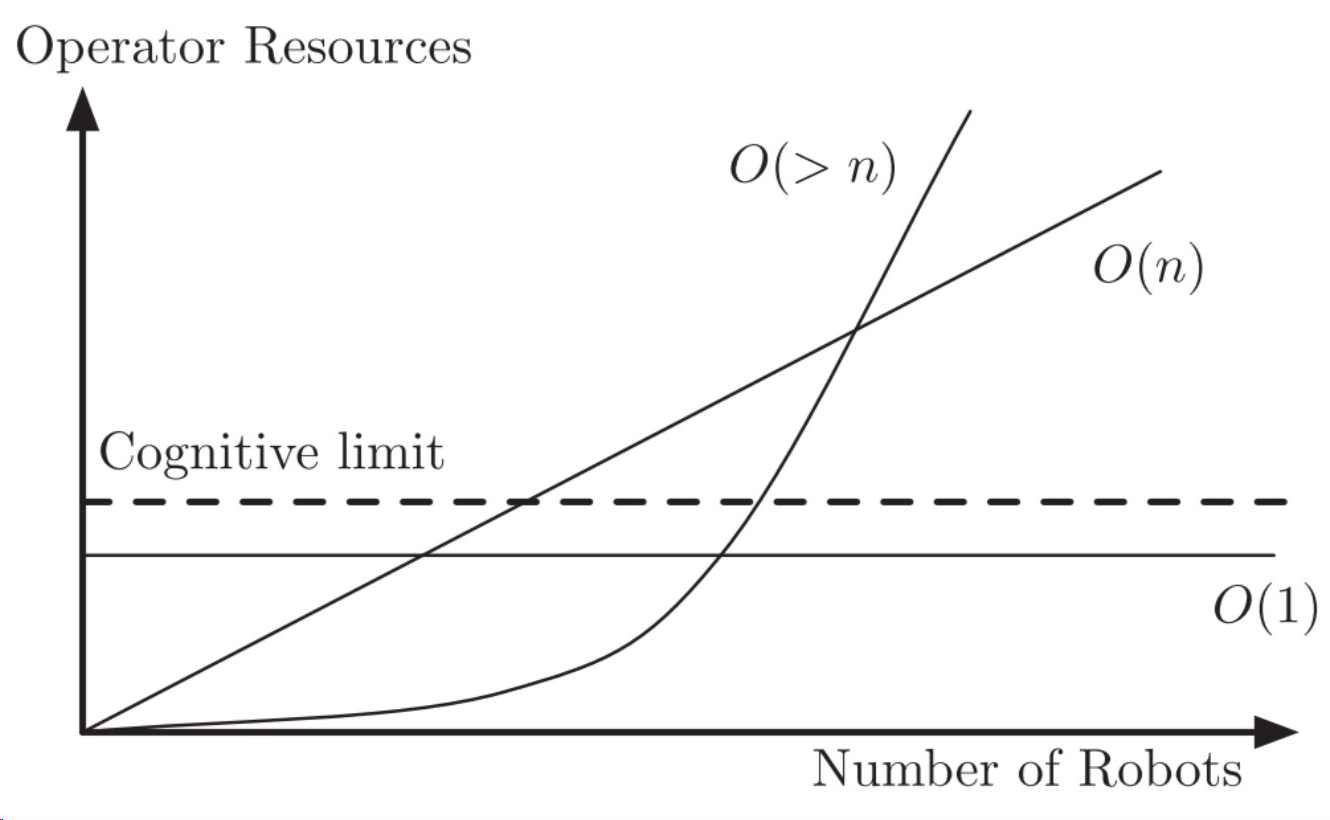
\includegraphics[width=0.8\linewidth]{figures/TradeStudy/figure2.png}
        \caption{Graphical illustration of the concept of control complexity in a human–multirobot system~\citep{kolling_human_2016}}
        \label{figure-hari:controlcomplexity}
    \end{center}
\end{figure}

Ongoing research into human-swarm interaction and multi-robot systems has primarily focused on coordinated swarm control, changing swarm topology, and describing the state of the swarm in a more understandable way~\citep{wang_current_2018}.
The development and design of human-swarm interfaces for multi-robot collaboration and, particularly, unmanned aerial vehicle teams is another important set of ongoing research.
The ability for swarms to multitask, and the requirement for the human operator to quickly task switch has been shown to cause detrimental effects on overall system performance~\citep{chen_humanagent_2014}.
High workload phases have been shown to be most sensitive to interruptions from tasks switching, suggesting that task switching should be avoided during these phases unless absolutely necessary~\citep{norman_user_1986}.
Issues relating to multitasking, task switching, and the loss of situational awareness can be mitigated with properly designed human-swarm interfaces.
Chen and Barnes outlined several of the prominent issues in user interface design and offered solutions in the form of guidelines~\citep{chen_humanagent_2014}.
They identified six issues range from ``maintaining operator's ultimate decision authority" to ``visualization and training techniques enhance human-agent collaboration", and present guidelines based on the findings of their review.

The concept of robots and automation systems that rely on externally networked support has also been explored by researchers~\citep{kehoe_survey_2015}.
New topics of research using ``the cloud" or otherwise networked robotics include big data, cloud computing, collective robot learning, and human computation, see Figure~\ref{figure-hari:cloudrobotics}.
Other key technologies which can be enhanced with networked robotic systems include human-robot collaboration technology, autonomous navigation technology under non-structured environments, multi-agent robot systems (swarms), and emotion recognition and interaction mechanism of robot oriented to harmonious human-robot cooperation~\citep{wang_current_2018}.
Issues associated with the rise in cloud technology include the need for techniques to consider time varying latency and quality of service, system security from remote intrusion, privacy concerns, and big data cleaning and filtering techniques.
Currently, cloud computing can be described as a framework with consists of three levels: Infrastructure as a Service (IaaS), where bare operating systems are available; Platform as a Service (PaaS), where more structure is provided, including access to application frameworks, databases, and programming languages; and Software as a Service (SaaS), where software is made available online rather than as a local service~\citep{kehoe_survey_2015}.

\begin{figure}[b!]
    \begin{center}
        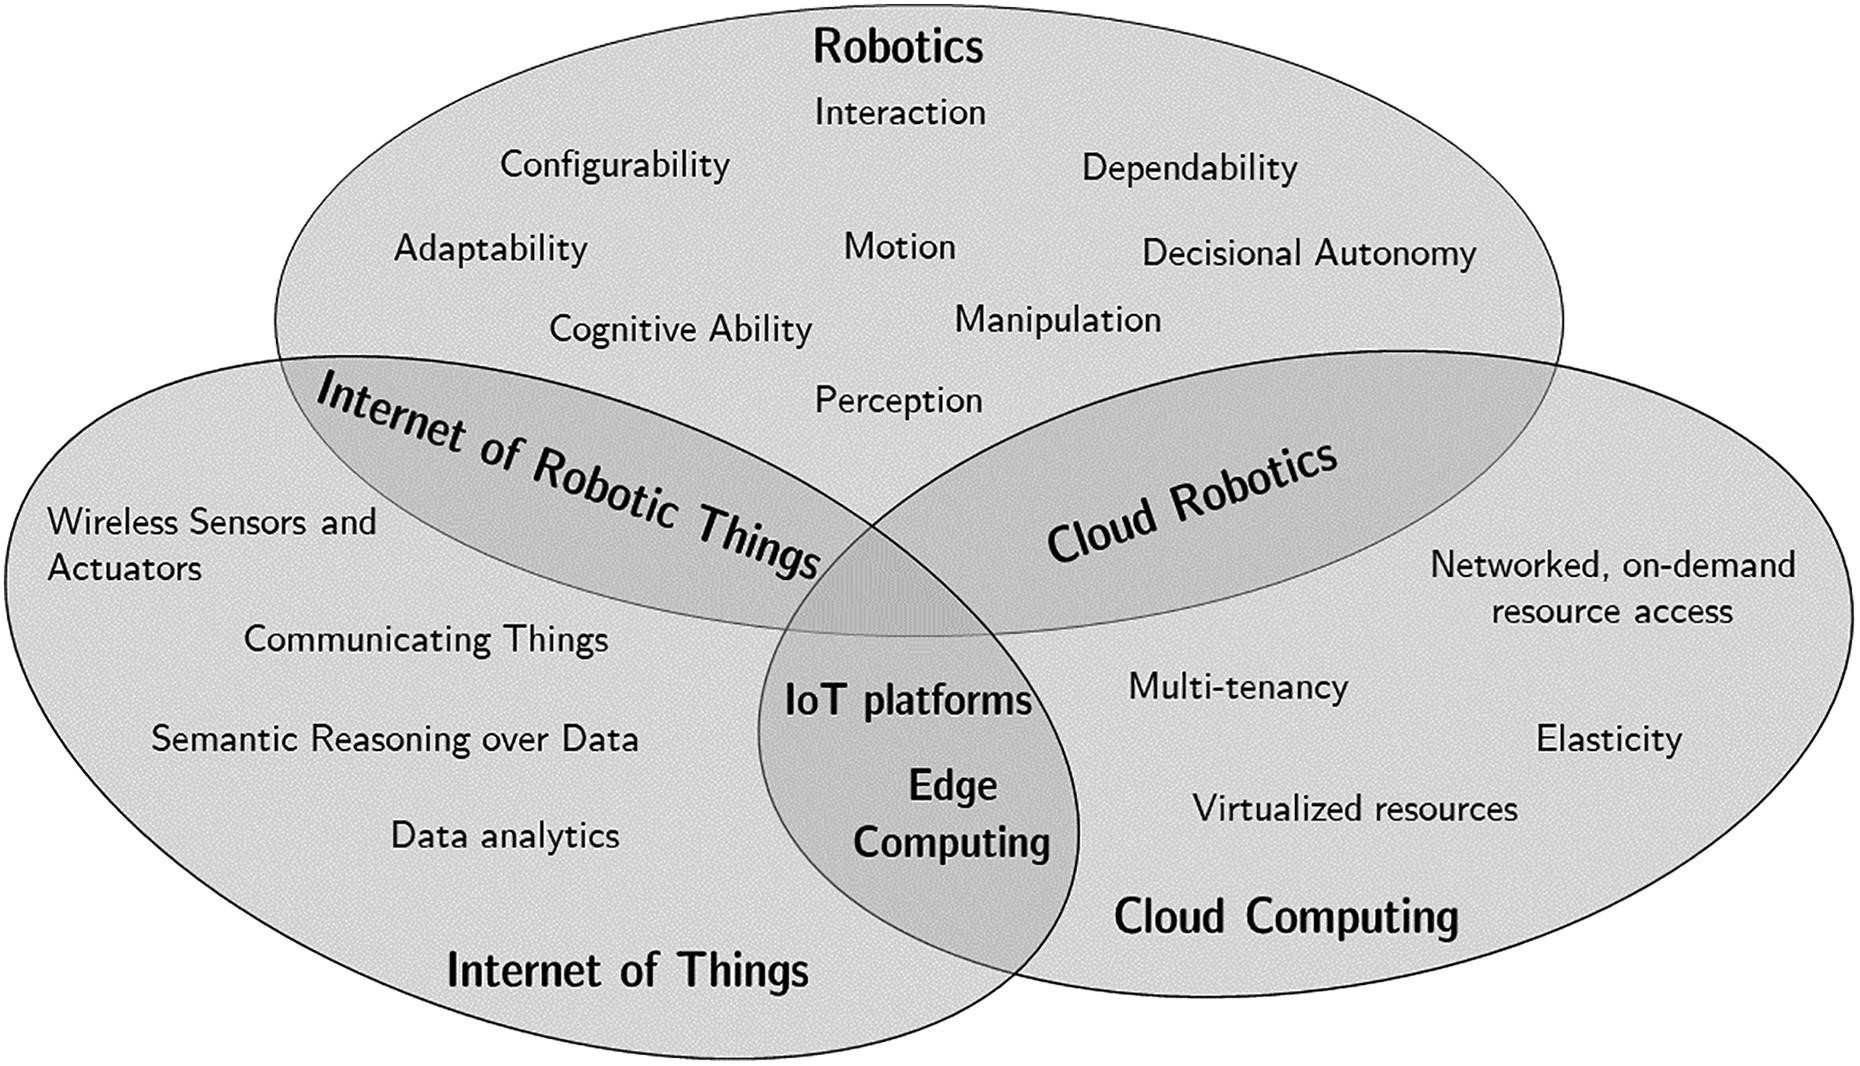
\includegraphics[width=0.8\linewidth]{figures/TradeStudy/figure3.jpg}
        \caption{Combining Robotics, the Internet of Things, and Cloud computing has resulted in many new possibilities such as Cloud Robotics~\citep{simoens_internet_2018}}
        \label{figure-hari:cloudrobotics}
    \end{center}
\end{figure}

\subsubsection{Trust}
Human trust has numerous definitions but for our purposes can be considered to be ``the attitude that an agent will help achieve an individual's goals in a situation characterized by uncertainty and vulnerability''~\citep{lee_trust_2004}.
Trust has become an increasing topic of research as robotics increasingly moves out of traditional settings such as manufacturing and into more common-place locations such as the office and the home.
Trust has a large impact on the physical safety of people operating around robots, as improper trust can lead a person to inadvertently place themselves in harm's way.
Considering the ways that trust changes over time has been an important aspect of the research into trust, and Schaefer et al. define trust as a three-dimensional expression of a relational property:
\begin{enumerate}
    \item An individual's overall, long-term propensity to trust in general
    \item A transient, momentary trust responsive to immediate ambient conditions
    \item How 1) and 2) evolve over time~\citep{schaefer_meta-analysis_2016}
\end{enumerate}
Their meta-analysis found strong effects between human-robot interaction and analyzed the factors that determine trust.
A robot or robotic system's ability to garner trust relies on several factors.
See Figure~\ref{figure-hari:trust} for Schaefer et al.'s conceptual organization of influencing the development of trust.
Trust is commonly assessed using surveys, many of which have been proposed, which attempt to measure the individual factors which establish trust.
These scales attempt to measure individual elements of trust, asking about the operator's assessment of the automation's competence, predictability, and dependability, among other factors.
Of these measurement techniques, two of the most commonly used scales are the ``Checklist for Trust between People and Automation''~\citep{jian_foundations_2000} and versions of Muir and Moray's subjective rating scales~\citep{muir_trust_1996}, though research into real-time techniques is ongoing~\citep{SEPPELT201966}.
Appropriate trust is important when shared control between human-robot teams is essential, as the human is more likely to arbitrate additional tasks to the robot when this trust is established~\citep{losey_review_2018}.

\begin{figure}[b!]
    \begin{center}
        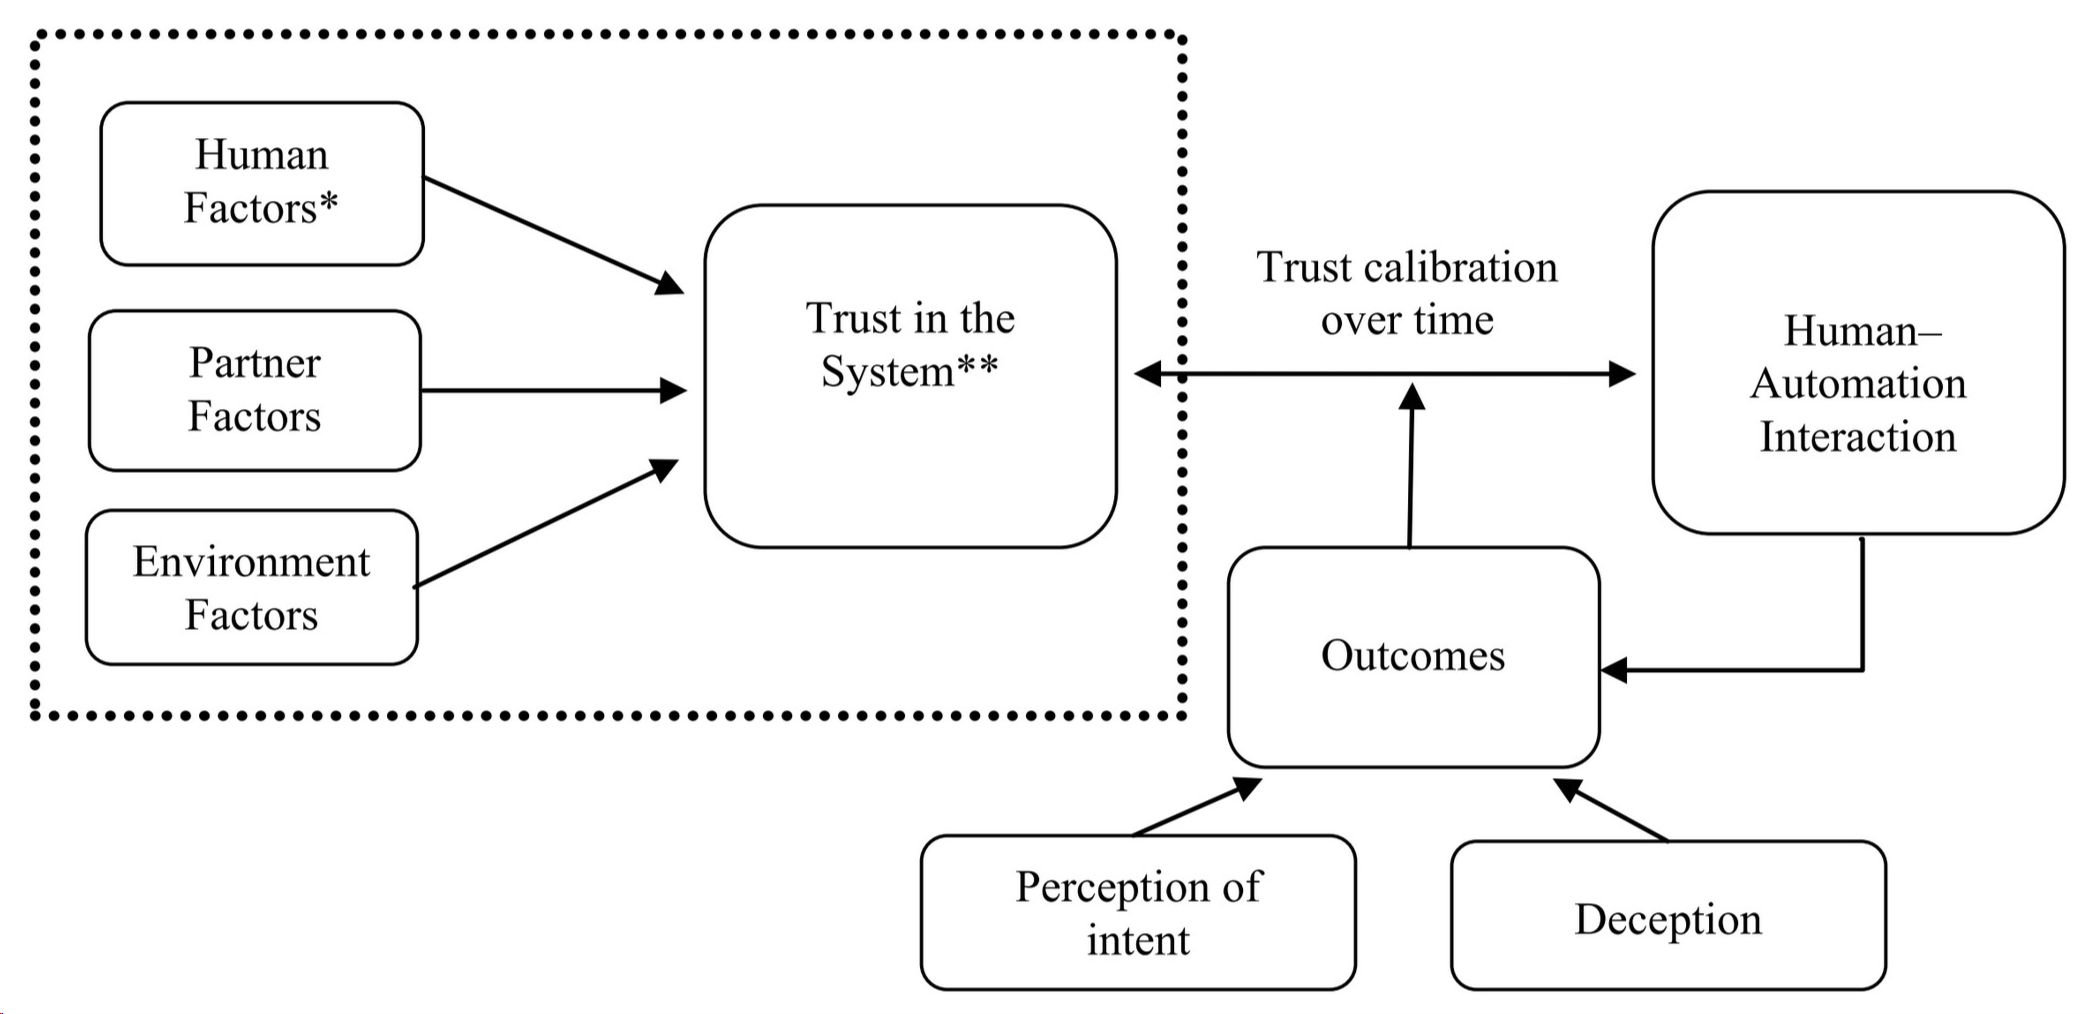
\includegraphics[width=0.8\linewidth]{figures/TradeStudy/figure4.png}
        \caption{A conceptual organization of trust influences highlighting trust development~\citep{schaefer_meta-analysis_2016}}
        \label{figure-hari:trust}
    \end{center}
\end{figure}

Ososky et al. made several propositions regarding human trust of robotics, among the most important being that:
\begin{itemize}
    \item Humans are easily influenced by superficial characteristics of robots
    \item Human subjective assessment of trust in robots ultimately determines the use of robotic systems~\citep{ososky_building_2013}
\end{itemize}
They noted that robot characteristics had the strongest influence on trust in human-robot teams, which included factors such as reliability, transparency, and anthropomorphic qualities.
One example of this is de Visser et al.'s 2016 study, which found that anthropomorphic automation associated greater trust resilience~\citep{de_visser_almost_2016}.
de Visser et al. concluded their study by suggesting that designers incorporate these features into future robots as a deliberate design choice to garner greater trust.
Even very simple additions such as high levels of mutual gaze have been shown to increase trust, while gaze aversions stoke feelings of distrust between human-robotic teams~\citep{admoni_social_2017}.

While anthropomorphism can lead to greater trust, some authors note caution when incorporating these features.
Culley and Madhaven warn that individual differences can lead some individuals to place too great a trust in anthropomorphic robots~\citep{culley_note_2013}.
Individuals are even more likely to trust anthropomorphic robots if they perceive similarities to the robot and themselves regarding age, gender, and even similarity of movement~\citep{pak_multi-level_2014, verberne_trusting_2013}.
Ososky further warns that trust in a robot's reliability alone is insufficient for better teamwork, and that over-trust combined with an inaccurate or incomplete mental model can lead to worse overall performance.
This is especially important when considering changing levels of automation in the field of human-automation interaction, for example, as an operator may not fully understand what they are currently responsible for, if the robotic system is in control.
This has led to numerous incidents leading to serious injury and death.
Trust in human-robot teaming is slightly different than trust in automation, however, as robots are often seen as collaborating teammates rather than just an automated tool~\citep{ososky_building_2013}.

\subsection{Interviews with Subject Matter Experts}
In order to provide a current assessment of the critical challenges associated with effective HARI systems across industries and domains, we also interviewed subject matter experts (SMEs).
SMEs were chosen to represent a cross section of HARI related disciplines such as aerospace, industrial robotics, military applications, medical, and autonomous vehicles.
SMEs were intentionally selected from different backgrounds, including military research, academia, and industry (robotics, medical, aerospace), in order to provide broad perspectives on the risks and challenges facing HARI technology development, as well as HARI technology and research.
We conducted ten phone interviews with SMEs who integrate humans, automation, and robotics in their work.
These interviews generally took between twenty and forty minutes.
We asked each expert the following questions:
\begin{enumerate}
    \item What technologies do you think are on the horizon in your field in the integration of humans, automation, and robotics?
    \item How would you prioritize what technologies are in development involving the integration of humans, automation, and robotics?
          \begin{enumerate}
              \item What technologies would be the most responsive to increased research support?
              \item For these technologies, what are the current TRLs? How much effort do you think it will take to raise the TRL over time?
          \end{enumerate}
    \item What are you most concerned about for the integration of humans, automation, and robotics? What technologies do you think could mitigate these risks?
          \begin{enumerate}
              \item What risks do you see arising from inclusion of these technologies (what new risks do you anticipate)?
              \item What risks currently have no technology solutions?
          \end{enumerate}
    \item How will these technologies fill the gaps in our current abilities?
          \begin{enumerate}
              \item Where do you see additional automation as a plausible way to fill those gaps?
              \item What other technology gaps should we be concerned about?
          \end{enumerate}
    \item Based on this discussion, is there anything else we should know?
\end{enumerate}

Based on the information gathered from literature and discussion with subject matter experts, the following specific HARI-related technologies and research topics emerged as areas for future research and development for the advancement of human automation and robotic interaction relevant to human spaceflight.

\subsection{Specific Technologies}
\subsubsection{Non-invasive behavioral and physiological sensing}
Non-invasive behavioral and physiological sensing includes a range of techniques.
Some physiological sensing techniques include common place, if controversial, methods such as a polygraph, to electromyography (EMG), electroencephalogram (EEG), and electrocardiogram (EKG) sensing.
Behavioral analysis techniques can include techniques that rely extensively on video analysis, such as gait analysis, and more integrated technology covering additional modalities.
This technology can be used to infer team member states.
The use of artificial intelligence to combine these perceptions is relatively developed.
This technology has an estimated TRL range of 3-5.

\subsubsection{Implantable Biometrics}
Compared to many of the other specific technologies we identified, implantable biometrics is a relatively young field which focuses on implantable biosensors for precision and personalized medicine.
These sensors can provide continuous data on specific, targeted metrics which can allow for the immediate detection of problems or need for intervention.
Implantable biometrics is especially important in the ``diagnosis, monitoring, management and treatment of a variety of disease conditions" and can be used to detect changes in a person's health~\citep{fitts_human_1951}.
Further advances in miniaturization and nanotechnology are likely needed for this technology to advance further.
This technology has an estimated TRL less than 3.

\subsubsection{Autonomous obstacle detection/imaging}
Autonomous obstacle detection/imaging is a combination of technologies designed to identify obstacles around a robot or other autonomous agent.
Detection and imaging can make use of visual spectrum or other light sources, acoustic or magnetic sensors, or laser-based technologies such as LIDAR.
Multiple techniques also take advantage of combining these technologies into multispectral sensors.
These technologies are important for autonomous docking and landing of spacecraft but have also seen an enormous increase in interest from the self-driving car industry.
One important side effect of increased demand of this technology in self-driving cars in the past few years is that the hardware has both rapidly miniaturized and dropped in price.
Note that this technology is only concerned with detection, while resulting actions and path planning is captured elsewhere (autonomous path planning).
This technology has an estimated TRL of 6 or greater.

\subsubsection{Autonomous path planning}
In contrast to autonomous obstacle detection, autonomous path planning describes the resultant planning and action that is taken after an obstacle is sensed or an objective is determined.
This technology benefits greatly from a good understanding of the robot or autonomous agent's dynamics, the environment it acts in, other agents in the environment, and the objective's location.
With regards to spaceflight, autonomous path planning is relevant when considering orbital proximity operations (including rendezvous and docking), surface landings, and rover movements.
This technology has also seen great benefits from the self-driving car industry, especially regarding planning around other moving agents whose intent is often poorly understood.
This technology has an estimated TRL of 6 or greater.

\subsubsection{Speech recognition}
Speech recognition is a set of technologies that enable the translation of spoken words to text by computer software.
Speech recognition has been actively developed since the 1970s and has a generally high rate of success.
Despite this relatively long period of development, recent advancements in speech recognition have been made by integrating machine learning techniques.
Transforming spoken word to text allows autonomous systems and robots to accept commands or infer human intent and is a common alternative to physical computer interfaces~\citep{tsarouchi_humanrobot_2016}.
It also allows for the detection of speech patterns and inflection classification to capture intent, trust, fatigue, or emotional states.
Depending on the system and application, speech recognition systems have higher TRL in the range of 6 or greater.

\subsubsection{Intuitive control interfaces}
Intuitive control interfaces consider ways of intuitively mapping human gestures to a resultant robotic action, and often takes human physiology, kinematics, and other elements of physical movement into consideration.
This technology includes interfaces types such as joysticks, keyboards, touchscreens, and gesture recognition, among others.
This technology has an estimated TRL of 6 or greater.

\subsubsection{Robotic/human information interfaces}
Information displays must determine what information to transmit for any given task, which may be customized based on user preference, task or environment concerns, past experiences, or the presence of anomalies.
These may include multimodal (visual, audio, and/or haptic) displays which display task relevant information to an operator.
They may display 2D or higher-dimensional information and may be body-worn or mounted in the environment.
These displays have elements designed by both human-computer interaction experts and machine learning algorithms.
Ideally, such displays would be ubiquitous, capable of quickly and easily transferring information between stations, and able to appear on traditional monitors, tablets, smartphones, or augmented reality interfaces.
While some elements are well-defined and arguably in use today, others remain in early stages of development.
Based on feedback, these systems have a current overall TRL estimated at 3-5.

\subsubsection{Augmented Reality and Virtual Reality}
Augmented and virtual reality are a pair of technologies which provide a partial or fully virtual environment to a user, often in the form of a head mounted display.
Augmented reality has also been developed to work with modern phones and tablets, and can provide additional, digital context to an otherwise physical object or environment.
Virtual reality is increasingly used as a training tool, while augmented reality has begun to be used as a tool for both training and operations.
This technology has an estimated TRL of 3-5.

\subsubsection{Robotic agents}
This technology encompasses a large variety of robots, which include rovers, satellite or UAV swarms, robotic arms, and vehicles, among others.
The relative TRL varies between relatively low, in the case of robotic swarms, to very high, in the case of rovers and robotic arms.
These sets of technologies enable humans to complete tasks that they could not otherwise accomplish, either because they take place in an extreme, dangerous or difficult to reach environment (as is the case with Martian rovers), they require abilities humans do not (moving payloads required by robotic arms such as Canadarm2) or because they would take too long (such as the mapping or scouting of a region by a swarm of UAVs or satellites).
On average, TRL may be estimated within the range of 3-5.

\subsubsection{Assistive Robotics}
In contrast to robotic agents, which largely replace the human or do not require a human to be present, assistive robotics describe robots that directly interface with humans to assist them in accomplishing a task.
These robots include small assistive satellites such as Astrobee, a modern version of the Apollo Lunar Roving Vehicle with more advanced guidance capabilities, exoskeletons, or personal assistants.
These robots enhance the already existing abilities of humans by enabling them to complete tasks that they otherwise could not, or by increasing performance in challenging tasks.
This technology has an estimated TRL of 3-5.

\subsubsection{Artificial Intelligence}
Artificial intelligence is intelligence demonstrated by machines, in contrast to human intelligence.
Some of the major goals of AI include knowledge reasoning, planning, natural language processing, computer vision, robotics, and machine learning.
In space HARI, AI could primarily be leveraged in managing complex systems (i.e. diagnostics, prognostics, and maintenance of spacecraft) and in acting as assistants for crew completing science and activity tasks.
By correctly interpreting human intent, AI can also control robots for payload and physical crew assistance.
This technology has an estimated TRL of 3-5.

\subsubsection{Machine Learning}
Machine learning describes a collection of algorithms which perform a specific task without using explicit instructions, instead relying on learned models.
Common types of machine learning include supervised learning, in which a human trains the model, unsupervised learning, where the system learns on its own, and reinforcement learning, where the software takes actions in an environment to optimize a cost function.
Machine learning has improved the performance of many varied technologies and is the foundation on which artificial intelligence is being developed upon.
This technology has an estimated TRL of 6 or greater.

\subsubsection{Flexible, Adaptive, or Adaptable Automation}
As noted earlier in the report, flexible, adaptive, and adaptable automation are widely praised in the literature for their ability to provide dynamic levels of automation.
The flexibility to provide different sets of automated features during different mission phases, for instance, is an effective requirement for many modern tasks.
Chen and Barnes define flexible automation as ``systems that invoke various levels of automation depending on the operator's state, critical events in the environment, or algorithms related to specialized problem sets"~\citep{chen_humanagent_2014}.
This technology has an estimated TRL of 6 or greater.

\subsection{Research Topics}
\subsubsection{Understanding human intent}
The topic of understanding human intent is wide, and includes subtopics such as the robotic interpretation of human intent, understanding human intent unobtrusively, and improving human to robot communication.
The interpretation of human intent by a computer or robot can be done in a variety of ways, including speech, gestures, and other forms of nonverbal communication.
These techniques are at varied levels of development, from basic proof of concept to use in operations.
Each technique can be broken down into several levels—gestures, for example, have four levels: sensor technologies, identification, tracking and classification~\citep{liu_gesture_2018}.
This is area is also closely tied to interpreting behavioral and human monitoring data and encompasses human/behavioral model research such as the prediction of intent from eye movements~\citep{Singh:2018:CPG:3237383.3237457, ruhland_review_2015}.

\subsubsection{Autonomous/robotic system communication to humans}
In contrast to the previous topic (understanding human intent) the research topic of autonomous/robotic system communication to humans addresses how these complex systems can best relay information back to a human operator.
This topic includes both research of communication techniques and mitigation of miscommunications from the system to the human.
This topic deals with discovering effective methods of providing information to a human user in an intuitive way, such that communication feels natural to a human operator.
Human-robot communication is largely focused on developing multisensory methods to successfully communicate a robot's intent to humans.
Human-autonomous system communications additionally deals with methods to successfully enable explainable and transparent autonomous system operation.

\subsubsection{Ensuring human safety (physical)}
This topic captures research which investigates how to enable safe human and robot operation in a shared environment in order to reduce risk.
It specifically investigates methods to successfully prevent harm to humans in close physical proximity with robots and develops guidelines and recommendations as to how physical interaction between robots and astronauts can safely occur.
This research topic benefits from the lessons learned in manufacturing settings, where humans and robots must often work nearby or directly with each other, as well as that work done by autonomous car companies in avoiding pedestrians.

\subsubsection{Continuous human performance monitoring}
The topic of continuous human performance monitoring seeks to understand human-system performance and measure human performance unobtrusively.
This research topic seeks to understand which human-system performance measures and limits are required for spaceflight and seeks to validate novel methods and technologies for measuring a variety of aspects of human performance such as task performance, workload, and situational awareness.
Research in this area also focuses on understanding the human performance effects resulting from adaptive automation and attempts to identify what are the performance differences between adaptable (human sets level of automation) versus adaptive (automation sets level of automation).

\subsubsection{HAR team performance optimization and function allocation}
Human autonomous/robotics team performance optimization and function allocation investigates different ways of understanding human-robot teamwork and human-autonomous system robustness, decides whether a particular function will be accomplished by a person, technology (hardware or software) or some mix of person and technology~\citep{fitts_human_1951}, and how to optimize that balance~\citep{yanco_analysis_2015}.
This research focuses on what social and teamwork elements enable successful human-robot collaboration, especially when it requires direct interaction between robots and astronauts.
With relation to robustness, this area also captures research on how to measure robustness when humans are using system in off-nominal conditions and identifying when these systems are off nominal.

\subsubsection{Enabling command/control of complex robotic systems}
This topic focuses on enabling command/control of complex robotic systems and enabling critical decision making.
This includes research on methods to successfully allow humans to command and control multiple, mixed robotic agents with varying levels of autonomy and flexible function allocation.
It also looks at new methods to enable humans to make time-critical decisions using autonomous systems across a variety of system dynamics and is required to evaluate methods for different autonomous systems with different functions (e.g., ECLSS vs. Power vs. Navigation).

\subsubsection{Improving situation awareness in HAR systems}
One of the most accepted definitions of situation awareness states that ``[s]ituation awareness is the perception of the elements in the environment within a volume of time and space, the comprehension of their meaning, and the projection of their status in the near future"~\citep{endsley2017toward}.
This research topic focuses on techniques to both maintain and improve operator situation awareness when interacting with automation/robotics systems.
Recent work by Endsley has further expanded early models of situation awareness, discussing the emerging problem of loss of operator situational awareness and out-of-the-loop performance problems associated with increasing system autonomy, reliability, and robustness~\citep{endsley_here_2017}.
This new model for human-autonomy system oversight (HASO), incorporates situation awareness, trust, workload and automation interfaces among the key system design features influencing human cognitive processes involved in successful interaction with automated systems.

\subsubsection{Improving training for HAR systems and tasks}
The topic of improving training for HAR systems and tasks investigates what new methods are required or most effective to train humans to use complex, advanced autonomous and robotic systems.
Research in this area explores different techniques and technologies to improve human performance and reduce workload, and often makes extensive use of mockups, simulations, hands-on walkthroughs, and human-in-the-loop studies.
Many techniques have been explored to improve training, including many kinds of feedback, manual control adaptation, and the use of virtual and augmented reality.

\subsubsection{Establishing appropriate trust in automation/robotics systems}
This research topic focuses on techniques to establish appropriate trust in automation/robotics systems and mitigating changes in trust between humans and these systems.
It explores how trust changes with factors such as communication, reliability, workload, social acceptability, privacy, and transparency.
As noted earlier, it can be challenging for operators to establish appropriate trust as these automation/robotics systems become more sophisticated~\citep{chen_humanagent_2014}.
This research has also focused on shared control between human-robot teams and how tasks are arbitrated to the robot when trust is established~\citep{losey_review_2018}.
Trust research investigates when there is a difference between expected and executed actions, and requirements on systems depending on whether knowledge is collected and maintained by software or by human operator.

\section{Trade Analysis}
In addition to specific technologies and research topics, the information gathered from the literature review and the discussions with subject matter experts was used to identify factors relevant to the assessment of technology or research for future investment.
With all of this information gathered, the factors were refined and used in a multi-dimensional trade study to assess the technologies and research topics as priorities for HARI investment.

\subsection{Factor Assessment with NASA Stakeholders}
In addition to interviewing the human, automation, and robotics integration SMEs, we also surveyed six NASA HARI stakeholders for their input on the trade study.
As NASA stakeholders involved in human, automation, and robotic interaction, we asked them to review eight factors and rank them from most important to least important in consideration of HARI technology for investment.
We also had them rank additional ``secondary criteria" for the factors related to risk.

Factors are characteristics of a technology that our team, in collaboration the NASA HARI DS, has identified and selected because they are relevant to assessing HARI.
These factors were generated from our review of the background literature and conversations with the SMEs.
NASA stakeholders were informed that these factors would be weighted and used to conduct a trade study designed to help NASA in prioritizing which technologies and, consequently, which HARI research areas, should be further invested in to help with future long duration exploration missions.
After our NASA stakeholders provided their input, we averaged and ranked their assessment of the factors.
The ranked factors appear in Table~\ref{table:factor-ranking}.

\begin{table}[tb]
    \centering
    \includetable{hari-factor-ranking.tex}
    \caption{The ranking of seven factors resulting from feedback from our NASA stakeholders}
    \label{table:factor-ranking}
\end{table}

\subsubsection{Task applicability}
Which tasks does the technology have an impact on? This factor characterizes how much impact the technology may have on the various HARI tasks identified for future exploration missions~\citep{marquez2017future}.
We determined if each technology applies to each task in order to measure the technology's applicability to space HARI.
These tasks, common to long duration orbital missions, deep space surface exploration missions, or both, are shown in Table~\ref{table:har-tasks}.

\begin{table}[tb]
    \centering
    \includetable{hari-har-tasks.tex}
    \caption{HAR tasks for spaceflight}
    \label{table:har-tasks}
\end{table}

\subsubsection{Task enabling}
Does the technology enable a new capability? This factor describes how much the technology enables one or more of the various HARI tasks identified for future exploration missions.
HARI tasks are assumed to be critical and must be completed.
We subjectively rated this by classifying the technology as: No effect relative to current technology (score of 0), Improves performance of current capability (score of 1), or Adds new capability (score of 2).

\subsubsection{Potential for reducing risk}
What is the benefit from risk reduction? This factor describes how risk might be reduced by the inclusion of the technology.
Each type of risk was subjectively rated.
Types of risks (secondary criteria) are listed below:
\begin{itemize}
    \item Improved safety: increase astronauts' safety.
    \item Reduced likelihood of system failure: increase overall robustness of system by predicting or preventing failures.
    \item Improved performance: astronauts can work more effectively and efficiently, including reducing physical and cognitive workload.
\end{itemize}

\subsubsection{Potential for introducing risk}
What is the cost from introduced risk? This factor describes how risk might be introduced by the inclusion of the technology.
Each type of risk was subjectively rated.
Types of risks are paired with the types of risk reduction.
Note that, unlike all the other factors, a higher potential for introducing risk has a negative impact on the technologies overall score.

\subsubsection{External investment (outside NASA)}
What is the current research activity going on outside of NASA? This factor characterizes how much research and investment has recently and is currently going into the development of the technology by entities outside of NASA.
This is just research on the technology, not HARI research investments.
We measured this using the publication rate associated with each technology.
The name of each technology was searched for on 6/24/2019 on Web of Science using the following search, where technology is substituted for each:
ALL FIELDS: (technology)
Timespan: 2013-2018.
Indexes: SCI-EXPANDED, SSCI, A\&HCI, CPCI-S, CPCI-SSH, BKCI-S, BKCI-SSH, ESCI, CCR-EXPANDED, IC.
Similarly, the technologies were also searched for in Google Scholar on the same date and with the same time span.
The sums from both searches were used to determine scores for this factor (see Trade Study Approach~\ref{ss:tsapproach}).

\subsubsection{Technology Readiness Level (TRL)}
What is the current TRL? This factor characterizes the maturity level of the technology.
We estimated the technology's current TRL using information gathered from the literature and provided by our SMEs.
TRL was split into three categories: Below TRL 3, TRL 3-5, and TRL 6 or greater.

\subsubsection{Research interest (within NASA)}
What is the current research interest within NASA? This factor describes if the technology has any potential for infusion into NASA missions as determined by the NASA Technology roadmaps/NASA Strategic Technology Investment Plan.
We qualify this by checking if the technology is present on the NASA technology roadmap.

\subsection{Trade Study Approach} \label{ss:tsapproach}
A multi-dimensional trade analysis was performed to objectively score HARI research topics and specific technologies in a recommended order of priority for NASA investment.
The approach used was similar to a Relationship Matrix Decomposition Scheme (RMDS)~\citep{boppe_training}, see Figure~\ref{figure-hari:tradestudy}.
The factors for assessment described above pertain directly to HARI technologies, while research topics are assessed through direct relationships with those technologies, see Figure~\ref{figure-hari:tradestudyA}.
This parallels the RMDS approach of tracing assessment of system configurations and technology options based on objectives/goals through functional options, see Figure~\ref{figure-hari:tradestudyB}.
For the complete trade table used in this study, see Appendix~\ref{appendix:trade-tables}.

\begin{figure}[tb!]
    \begin{center}
        \begin{subfigure}{0.49\textwidth}
            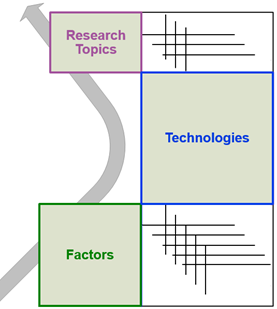
\includegraphics[width=\linewidth]{figures/TradeStudy/figure5a.png}
            \caption{Top-level trade study approach used in the HARI analysis}
            \label{figure-hari:tradestudyA}
        \end{subfigure}\hfill
        \begin{subfigure}{0.49\textwidth}
            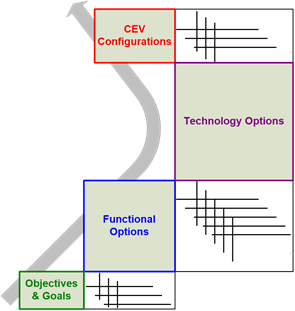
\includegraphics[width=\linewidth]{figures/TradeStudy/figure5b.png}
            \caption{Structure of the RMDS trade study approach}
            \label{figure-hari:tradestudyB}
        \end{subfigure}
        \caption{Trade study approaches}
        \label{figure-hari:tradestudy}
    \end{center}
\end{figure}

Research topics and technologies were defined as related if a given technology supports the research topic such that its development would fundamentally drive investigation of that topic.
Each technology was given a score resulting from the technology-factors dimension of the trade.
The scores for each related technology for a given research topic were summed to achieve the total score for that topic.

The technology total scores represent a roll-up of individual weighted factor scores for each specific technology.
At a factor level, normalized scores for each technology were determined in a series of one-dimensional factor-technology trade studies.
These individual factor-level trades used to compile the factor-technology dimension are found in Appendix~\ref{appendix:trade-tables}.
The factor scores were multiplied by the factor weights as defined in the NASA Stakeholders section of this report and summed for each technology.

\subsubsection{Factor-Level Trades}
The factor-level trades for Risk Reduced, Risk Introduced, and TRL each assessed the specific technologies against three weighted options.
Risk Reduced, for example assigned an individual score of 0 or 1 to each technology if it potentially reduced risk to crew, risk to mission/vehicle, or risk of loss of performance.
Each potentially reduced risk was weighted (1 to 3) based on relative ranking as found by the NASA stakeholders.
The total weighted scores for each technology (sum of weights x scores) were normalized by the highest possible score for a single technology to find the factor scores on a scale between 0 and 1 (see Equation~\ref{eq:weighted-score}, below).

\begin{align}
    \mbox{Normalized Score} =  \frac{{\Sigma}(\mbox{Weighted Scores for a Technology})}{{\Sigma}(\mbox{Weights}) \times \max(\mbox{Individual Score})}
    \label{eq:weighted-score}
\end{align}

For Risk Introduced, normalized scores were multiplied by -1, as introduced risk were tallied as a negative contribution to overall technology assessment.
The TRL trade was performed identically to Reduced Risk, with the exception that technologies could only be assigned to a single average TRL range.
Assessment for Research Interest (within NASA) was simplified compared to other factor-level trades as scoring had a single binary level (trade table included in Appendix~\ref{appendix:trade-tables}).

In the Task Applicability and Task Enabling factor-level trades, scores were assigned between technology and task, with equal weighting across tasks (all assigned a weight of 1).
Technologies were assessed for Task Applicability with a score of 0 or 1, while for Task Enabling technologies were assigned a score for each task of 0, 1, or 2 as described in the NASA Stakeholders section.

In assessment of External Investment in NASA, as described previously, two search engines were used to find estimates on the number of recent publications pertaining to each technology.
Searches with each service are known to poll databases of drastically different size.
The relative database size used by both search engines was accounted for by applying a weight determined by the largest publication total found for each service.
In this way, the relative publication totals for each service could be normalized independently prior to summing the results of the two searches.

\section{Results}

\subsection{Research Topics}
The final scores for research topics have been ranked, such that a high score represents a recommended higher priority for research investment by NASA (see Table~\ref{table:topic-prioritization}).
The top-ranking research topics are:
\begin{enumerate}
    \item Improving training for HAR systems and tasks
    \item Establishing appropriate trust in automation/robotics systems
    \item Understanding human intent
\end{enumerate}

\begin{table}[tb]
    \centering
    \includetable{hari-topic-prioritization.tex}
    \caption{The resulting prioritization of research topics from linking research topics to the upcoming technologies}
    \label{table:topic-prioritization}
\end{table}

Note that all these topics were identified as areas applicable to HARI concerns, regardless of the score.
A high score here is highly dependent on the impact of the surveyed technologies on the research topic and suggests which research topics should be able to make relatively quick progress given the technology that is being developed now and in the next 5-10 years.
A low score reflects research topics that either have relatively few technology solutions on the horizon, had relatively low factor scores for the technologies that are related to the topic, or both.

These top-ranking research topics were driven by their associated highly scoring technologies.
Improving training for HAR systems and tasks touches on a variety of upcoming technologies ranging from machine learning to robotic/human information interfaces.
These technologies ranked highly in their task applicability and potential for reducing risk and had relatively little potential for introducing new risks when compared to other technologies.
By leveraging these upcoming technologies, researchers have ample opportunities to investigate novel techniques for improving training for these systems.
These upcoming techniques will prove invaluable as HAR systems and tasks continue to increase in complexity, especially if, for example, they can provide crew with just-in-time training for critical tasks when they are far from the support provided by mission control.
The topic of training came up many times in our conversations with subject matter experts, who often noted case examples of major failures in their explanations for why this training was needed.
Similarly, many subject matter experts also mentioned the need for establishing appropriate trust in automation/robotics systems during our interviews, a topic which came up repeatedly in our review of the literature.
Over-trust and under-trust in these complex systems were both noted as being dangerous and can result from inadequate training.
Research in trust has often focused on its role in flexible, adaptive, and adaptable automation, where operators can be unclear which mode the system is in.
By taking advantage of upcoming technologies in intuitive physical control and robotic/human information interfaces, researchers can help to bring humans into the loop on what is happening within these complex systems.

In contrast to the top-ranking research topics, continuous human performance monitoring and improving situation awareness in HAR systems were among the lowest ranked topics.
While both are important when considering future long duration exploration missions, neither were directly associated with many upcoming technologies.
Despite being associated with the top-ranking technology, machine learning, continuous human performance monitoring ranked lowest.
This is primarily because it was also associated with the two lowest ranking technologies, non-invasive behavioral and physiological sensing and implantable biometrics.
Despite these technologies' clear relation to performance monitoring, they were among the lowest ranking when considering the task applicability and task enabling factors, which were considered the most important by our NASA stakeholders.
Improving situation awareness in HAR systems lower score came as a surprise as situation awareness presents a challenge across all HAR applications.
Although it also benefited from being linked to a top-ranking technology—robotic/human information interfaces—but the topic otherwise suffered from few direct technology solutions.

\subsection{Technologies}
The resulting ranks of the technologies from the weighted factors are shown in Table~\ref{table:technology-prioritization}.
The top-ranking technologies identified from the trade study are:
\begin{enumerate}
    \item Machine Learning
    \item Autonomous obstacle detection/imaging
    \item Robotic/human information interfaces
    \item Artificial Intelligence
\end{enumerate}

\begin{table}[tb]
    \centering
    \includetable{hari-technology-prioritization.tex}
    \caption{The resulting prioritization of technologies using the trade study}
    \label{table:technology-prioritization}
\end{table}

These top-ranking technologies have seen enormous advancements in research interest and development over the past few years, and all offer a large benefit to the tasks required by NASA on future LDEMs.
In contrast to the top-ranking technologies, low ranking technologies show a trend of reflecting a combination of low research interest, task relevance, or TRL.

The top-ranking technologies all benefited from high marks across all our factors.
Machine learning, our top-ranking technology, particularly stands out due to scoring highest in the External Investment (outside of NASA) factor, where it significantly outperformed the other technologies.
As we noted in the literature review, machine learning came has been repeatedly forecast as being essential to the future of human-robotic interaction~\citep{wang_current_2018}.
It also came up extensively in our conversations with our subject matter experts, though several of these also stressed caution in assuming machine learning could solve any problem without issue.
Artificial Intelligence was also mentioned by most of the SMEs but ranked lower due to its dramatically higher potential for introducing risk.

Autonomous obstacle detection/imaging was our second highest scoring factor but had little impact on our research topic recommendations.
Despite being a well-established technology, the only topic is was ultimately related to was ensuring human safety (physical).
Like our other high scoring technologies, however, it scored well due to its high task applicability, task enabling potential for reducing risk factors.
This suggests that, while the technology should continue to be developed and refined, there is minimal applicability toward ongoing research that addresses outstanding HARI risks and challenges.
Improvements resulting from refinement in the commercial sector, especially regarding autonomous cars, should enable faster and safer algorithms in the future.

Several technologies were highly clustered in the middle of our rankings: autonomous path planning, augmented reality/virtual reality, robotic agents, and flexible/adaptive/adaptable automation also scored within a few tenths of a point from each other.
These technologies all had relatively high potential for introducing risk but were otherwise highly applicable to the tasks related to space HARI.
As noted previously, the two lowest ranking technologies, non-invasive behavioral and physiological sensing and implantable biometrics were among the lowest ranking when considering the task applicability and task enabling factors, which were considered the most important by our NASA stakeholders.
These technologies were also those which did not score in the Research Interest (within NASA) factor, as they were not present in the NASA Technology roadmaps or NASA Strategic Technology Investment Plan.
The third lowest ranking technology, speech recognition, despite being a widespread, high TRL technology, scored poorly because it was the lowest scoring in both the task applicability and task enabling factors.

\section{Contribution (Relation to NASA HARI Gaps)}
NASA has identified four gaps in HARI knowledge, as part of the larger HFBP characterization of human factors risks and associated knowledge gaps~\citep{hari_risk}.
These gaps need to be closed in order to mitigate HARI related risk as it pertains to spaceflight.
The NASA HARI Gaps are:
\begin{itemize}
    \item[\textbf{HARI-01}] We need to evaluate, develop, and validate methods and guidelines for identifying human-automation/robot task information needs, function allocation, and team composition for future long duration, long distance space missions.
    \item[\textbf{HARI-02}] We need to develop design guidelines for effective human-automation-robotic systems in operational environments that may include distributed, non-collocated adaptive mixed-agent teams with variable transmission latencies.
    \item[\textbf{HARI-03}] We do not know how to quantify overall human-automation-robotic system performance to inform and evaluate system designs to ensure safe and efficient space mission operations.
    \item[\textbf{HARI-04}] We need to identify and scope the critical human-automation/robotic mission activities and tasks that are required for future long duration, long distance space missions.
\end{itemize}

This study extends prior investigation of HARI tasks, specifically to address gap HARI-04 directly.
This investigation and trade study identify prioritized lists of specific technologies whose advancement support the activities and tasks required for future space exploration missions, as well as research topics where investment will support both HARI task capabilities and closing of the other three HARI knowledge gaps.
All the research topics identified in this report can assist with closing HARI-02, and most address HARI-03 as well.
Table~\ref{table:hari-gaps} provides a complete mapping of the relationships between with research topics and HARI gaps.
Although few of the research topics address HARI-01, the outstanding concerns identified by NASA for closer of HARI-01 pertain directly to the topics of safety and function allocation, which are reflected here.

\begin{table}[tb]
    \centering
    \includetable{hari-gaps.tex}
    \caption{Mapping of HARI related Research Topics to HARI Gaps identified by NASA}
    \label{table:hari-gaps}
\end{table}

\section{Recommendations}
Based on the trade analysis performed, we recommend that NASA's HFBP Element prioritizes research investment in the topics of improving training for HAR systems and tasks, establishing appropriate trust in autonomous/robotic systems, and understanding human intent.
It is important to note that all the identified HARI research topics have application toward mitigating HARI risk in spaceflight tasks for future missions.
These topics, however, represent the highest-priority areas for investment.

Investigation and identification of methods to improve training for HAR systems has the potential for far-reaching impact on reducing risk in mission operations, with limited chance of introducing new risk.
Training is also a ubiquitous concern across all HAR systems and tasks.
Similarly, establishing trust between the human and robotic/autonomous system showed trends of tracing to high risk reduction potential, though risk introduction potential was more varied.
Trust between the human and the autonomous system (or robotic agent) came up again and again in discussions with experts across different HARI related disciplines as critical to the success of HAR operations.
Without appropriate trust, elements fundamental to other research topics, such as teamwork or performance, break down.

While understanding human intent ranked highly as a research topic largely because of the number of technologies to which it was related, we believe this topic deserves its place in the prioritized rankings because, like training and establishment of trust, it stands out in overall potential to address HAR concerns for spaceflight.
The ability to interpret human communication, input, need, and general intent is critical to the successful operation of any HAR system which interacts directly with a human user.
Consequently, it is strongly tied to several of the other research topics defined (e.g. continuous human performance monitoring, enabling command/control of complex robotic systems) and investment in this area could bolster study in those lower-priority topics as well.

One of the primary outcomes from this research was to determine directions for HARI research that will close HARI risk and support capabilities for HAR tasks in space exploration.
Investigation of these research topics will provide a fundamental foundation for addressing challenges that face implementation of HARI technology solutions.
Improvement of training, trust, and human intent interpretation in HAR systems enables capability for a wide range of HAR space exploration tasks, both for long duration orbital missions and future planetary surface exploration.
